\documentclass[12pt]{article}
\usepackage[utf8]{inputenc}
\usepackage{float}
\usepackage{amsmath}

\usepackage[hmargin=3cm,vmargin=6.0cm]{geometry}
%\topmargin=0cm
\topmargin=-2cm
\addtolength{\textheight}{6.5cm}
\addtolength{\textwidth}{2.0cm}
%\setlength{\leftmargin}{-5cm}
\setlength{\oddsidemargin}{0.0cm}
\setlength{\evensidemargin}{0.0cm}

%misc libraries goes here
\usepackage{tikz}
\newcommand{\boldP}{\textbf{\textit{P}}}
\usepackage{graphicx}
\allowdisplaybreaks

\usepackage{listings}
\usepackage{xcolor}

\definecolor{codegreen}{rgb}{0,0.6,0}
\definecolor{codegray}{rgb}{0.5,0.5,0.5}
\definecolor{codepurple}{rgb}{0.58,0,0.82}
\definecolor{backcolour}{rgb}{0.95,0.95,0.92}

\lstdefinestyle{mystyle}{
  backgroundcolor=\color{backcolour},
  commentstyle=\color{codegreen},
  keywordstyle=\color{magenta},
  numberstyle=\tiny\color{codegray},
  stringstyle=\color{codepurple},
  basicstyle=\ttfamily\footnotesize,
  breakatwhitespace=false,
  breaklines=true,
  captionpos=b,
  keepspaces=true,
  numbers=none,
  numbersep=5pt,
  showspaces=false,
  showstringspaces=false,
  showtabs=false,
  tabsize=2
}

\lstset{style=myStyle}

\begin{document}

\section*{Student Information }
%Write your full name and id number between the colon and newline
%Put one empty space character after colon and before newline
Full Name : Murat Bolu \\
Id Number : 2521300 \\

% Write your answers below the section tags
\section*{Answer 1}

\subsection*{a)}

\begin{itemize}
  \item Since both $T_A$ and $T_B$ are uniformly distributed, their probability
  density functions are $f_A = f_B = \frac{1}{100}$ with $b = 100$ and $a = 0$.
  Since they are independent, the joint density function is $f(t_A, t_B) = f_A
  \cdot f_B = \frac{1}{10,000}$.
  \item The joint cumulative distribution function is $F(t_A, t_B) = \iint
  \frac{dx \cdot dy}{10,000} = \int \frac{x \cdot dy}{10,000} = \frac{x \cdot
  y}{10,000}$.
\end{itemize}

\subsection*{b)}

Let's draw a $100 \times 100$ square to illustrate the probabilites. Since the
probability density function is a constant function, the simple area of a region
over ten thousand would give us the probability of an event being inside the
region.

\begin{center}
  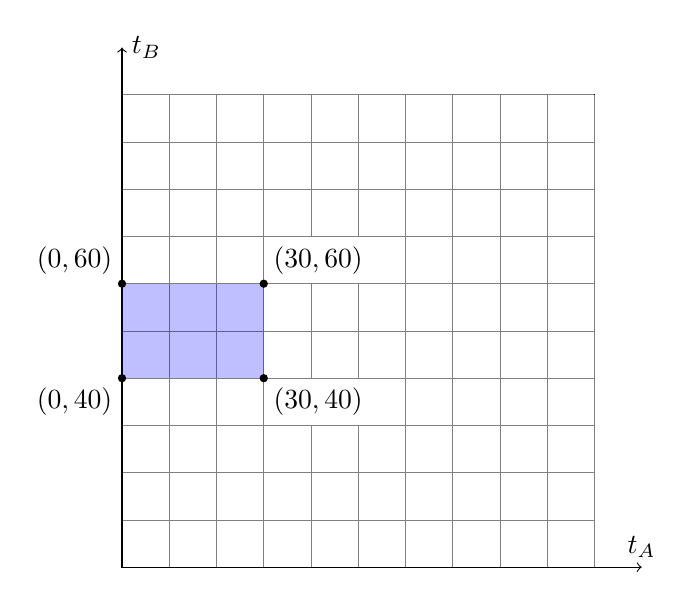
\begin{tikzpicture}[scale=0.6]
    \draw (0,0) rectangle (10,10);
    \draw [help lines] (0,0) grid (10,10);
    \draw [->] (0,0) -- (11,0) node [above] {$t_A$};
    \draw [->] (0,0) -- (0,11) node [right] {$t_B$};
    \fill [nearly transparent, blue] (0,4) -- (0, 6) -- (3,6) -- (3,4);
    \path (0,4) node [below left]  {$(0, 40)$}
          (0,6) node [above left]  {$(0, 60)$}
          (3,6) node [above right, fill=white] {$(30, 60)$}
          (3,4) node [below right, fill=white] {$(30, 40)$};
    \fill (0,4) circle [radius=2.5pt]
          (0,6) circle [radius=2.5pt]
          (3,6) circle [radius=2.5pt]
          (3,4) circle [radius=2.5pt];
  \end{tikzpicture}
\end{center}

\noindent
The blue region depicts the probability $P\{T_A < 30 \cap 40 < T_B < 60\}$. The
probability is equal to the volume of the space underneath it, where the space
is bounded by the probability density function $f$ from the above. Since $f$ is
constant, the volume simply equals to $30 \cdot 20 \cdot \frac{1}{10000} =
\frac{600}{10000} = \frac{3}{50} = 0.06$.

\newpage

\subsection*{c)}

For this question, we must calculate the area of the surface of square with the
constraint $t_A < t_B + 10$.

\begin{center}
  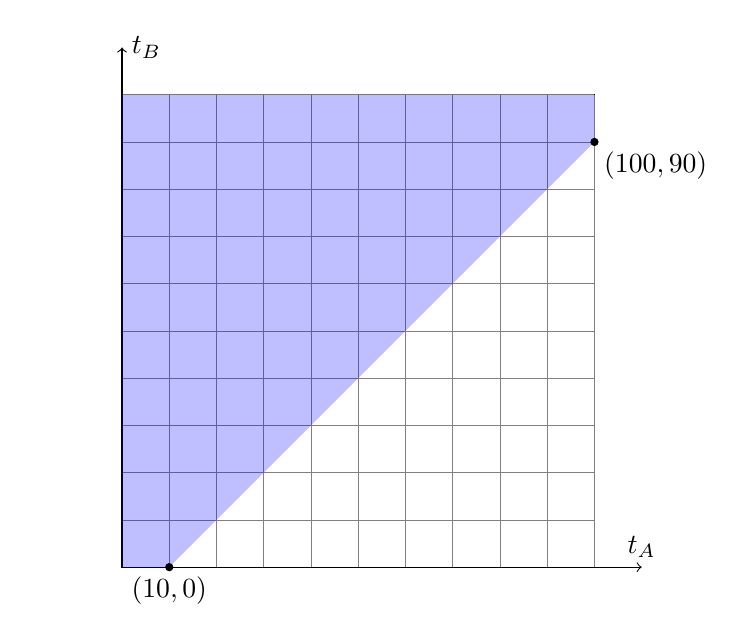
\begin{tikzpicture}[scale=0.6]
    \draw (0,0) rectangle (10,10);
    \draw [help lines] (0,0) grid (10,10);
    \draw [->] (0,0) -- (11,0) node [above] {$t_A$};
    \draw [->] (0,0) -- (0,11) node [right] {$t_B$};
    \fill [nearly transparent, blue]
      (1,0) -- (0,0) -- (0,10) -- (10, 10) -- (10,9) -- (1,0);
    \path (1,0)  node [below] {$(10, 0)$}
          (0,2)  node [transparent, left] {$(0, 20)$}
          (10,9) node [below right] {$(100, 90)$};
    \fill (1,0)  circle [radius=2.5pt]
          (10,9) circle [radius=2.5pt];
  \end{tikzpicture}
\end{center}

\noindent
The area of the surface is $100 \cdot 100 - 90 \cdot 90 \cdot \frac{1}{2} =
5950$. The volume of the space is $5950 \cdot \frac{1}{10000} =
\frac{5950}{10000} = \frac{119}{200} = 0.595$.

\subsection*{d)}

For this question, the inequality $|t_A - t_B| < 20$ must be satisfied. This
equals to $-20 < t_A - t_B < 20$ which means $t_B - 20 < t_A < t_B + 20$.

\begin{center}
  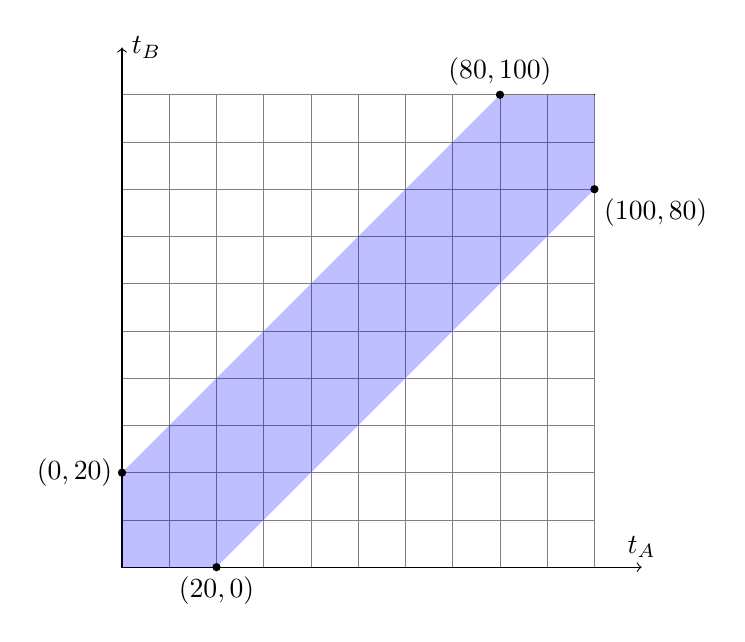
\begin{tikzpicture}[scale=0.6]
    \draw (0,0) rectangle (10,10);
    \draw [help lines] (0,0) grid (10,10);
    \draw [->] (0,0) -- (11,0) node [above] {$t_A$};
    \draw [->] (0,0) -- (0,11) node [right] {$t_B$};
    \fill [nearly transparent, blue]
      (2,0) -- (0,0) -- (0,2) -- (8, 10) -- (10,10) -- (10,8) -- (2,0);
    \path (2,0)  node [below] {$(20, 0)$}
          (0,2)  node [left] {$(0, 20)$}
          (10,8) node [below right] {$(100, 80)$}
          (8,10) node [above] {$(80, 100)$};
    \fill (2,0)  circle [radius=2.5pt]
          (0,2)  circle [radius=2.5pt]
          (10,8) circle [radius=2.5pt]
          (8,10) circle [radius=2.5pt];
  \end{tikzpicture}
\end{center}

\noindent
The area of the surface is $100 \cdot 100 - 2 \cdot 80 \cdot 80 \cdot
\frac{1}{2} = 3600$. The volume of the space is $3600 \cdot \frac{1}{10000} =
\frac{3600}{10000} = \frac{9}{25} = 0.36$.

\newpage

\section*{Answer 2}

\subsection*{a)}

This probability is binomially distributed with parameters $n = 150$, because
150 people are selected from the population, and $p = 0.6$, because frequent
shoppers are $60\%$ of the population. Since $n$ is large, normal approximation
to binomial distribution with parameters $\mu = n \cdot p$ and $\sigma = \sqrt{n
\cdot p \cdot (1 - p)}$ can be used. In that case, $\mu = 90$ and $\sigma = 6$.
In order for the $65\%$ of the customers to be frequent shoppers, at least 97.5
of them should be frequent shoppers.

\vspace{-5mm}
\begin{align*}
  \boldP\{X > 150 \cdot 0.65\}
    &= \boldP\{X > 97.5\} \\
    &= \boldP \left\{ \frac{X - 90}{6} > \frac{97.5 - 90}{6} \right\} \\
    &= \boldP \left\{ \frac{X - 90}{6} > \frac{7.5}{6} \right\} \\
    &= \boldP \left\{ \frac{X - 90}{6} > 1.25 \right\} \\
    &= 1 - \boldP \left\{ \frac{X - 90}{6} < 1.25 \right\} \\
    &= 1 - \Phi(1.25) \\
    &= \Phi(-1.25) \\
    &= 0.1056
\end{align*}

\subsection*{b)}

Similarly, this probability is binomially distributed with parameters $n = 150$,
and $p = 0.1$. Normal approximation has $\mu = 15$ and $\sigma = \sqrt{13.5} =
3.6742$ as parameters. At most 22.5 of customers must be rare shoppers.

\vspace{-5mm}
\begin{align*}
  \boldP\{X < 150 \cdot 0.15\}
    &= \boldP\{X < 22.5\} \\
    &= \boldP \left\{ \frac{X - 15}{\sqrt{13.5}}
                    < \frac{22.5 - 15}{\sqrt{13.5}} \right\} \\
    &= \boldP \left\{ \frac{X - 15}{\sqrt{13.5}}
                    < \frac{7.5}{\sqrt{13.5}} \right\} \\
    &= \boldP \left\{ \frac{X - 15}{\sqrt{13.5}} < 2.0412 \right\} \\
    &= \Phi(2.0412) \\
    &= 0.9794
\end{align*}

\newpage

\section*{Answer 3}

\begin{align*}
  \boldP\{170 < X < 180\}
    &= \boldP \left\{ \frac{170 - 175}{7}
                    < \frac{X - 175}{7} < \frac{180 - 175}{7} \right\} \\
    &= \boldP \left\{ -\frac{5}{7} < \frac{X - 175}{7} < \frac{5}{7} \right\} \\
    &= \boldP \left\{ -0.7143 < \frac{X - 175}{7} < 0.7143 \right\} \\
    &= \Phi(0.7143) - \Phi(-0.7143) \\
    &= 0.7625 - 0.2375 \\
    &= 0.5249
\end{align*}

\section*{Answer 4}

\subsection*{a)}

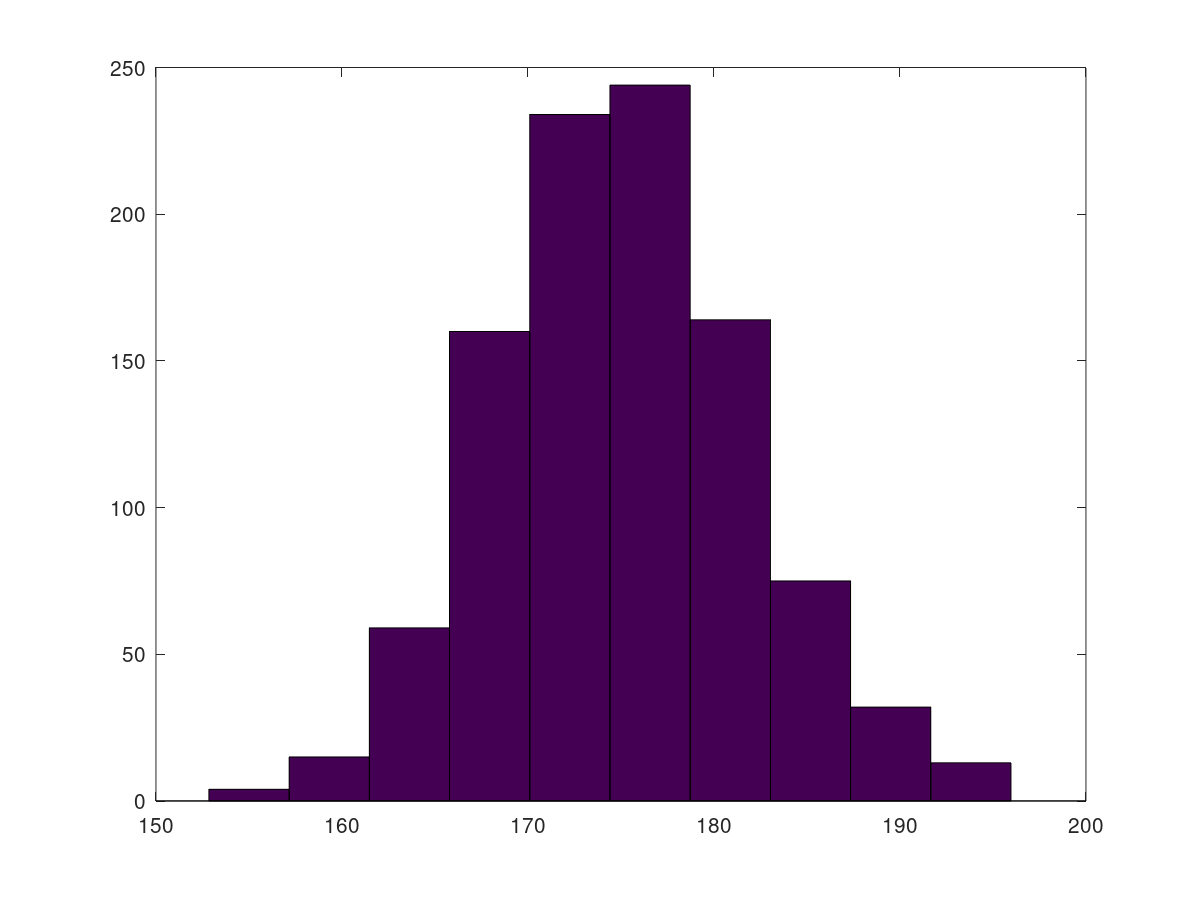
\includegraphics[width=\textwidth]{the2_hist.png}

The histogram of the data is similar to the probability density function of the
normal distribution, with parameters $\mu = 175$ and $\sigma = 7$. If we were to
make more trials and visualize the result with more bars, the resulting chart
would be closer to normal PDF. This is essentially Riemann sum of the integral
of the PDF.

\subsection*{b)}

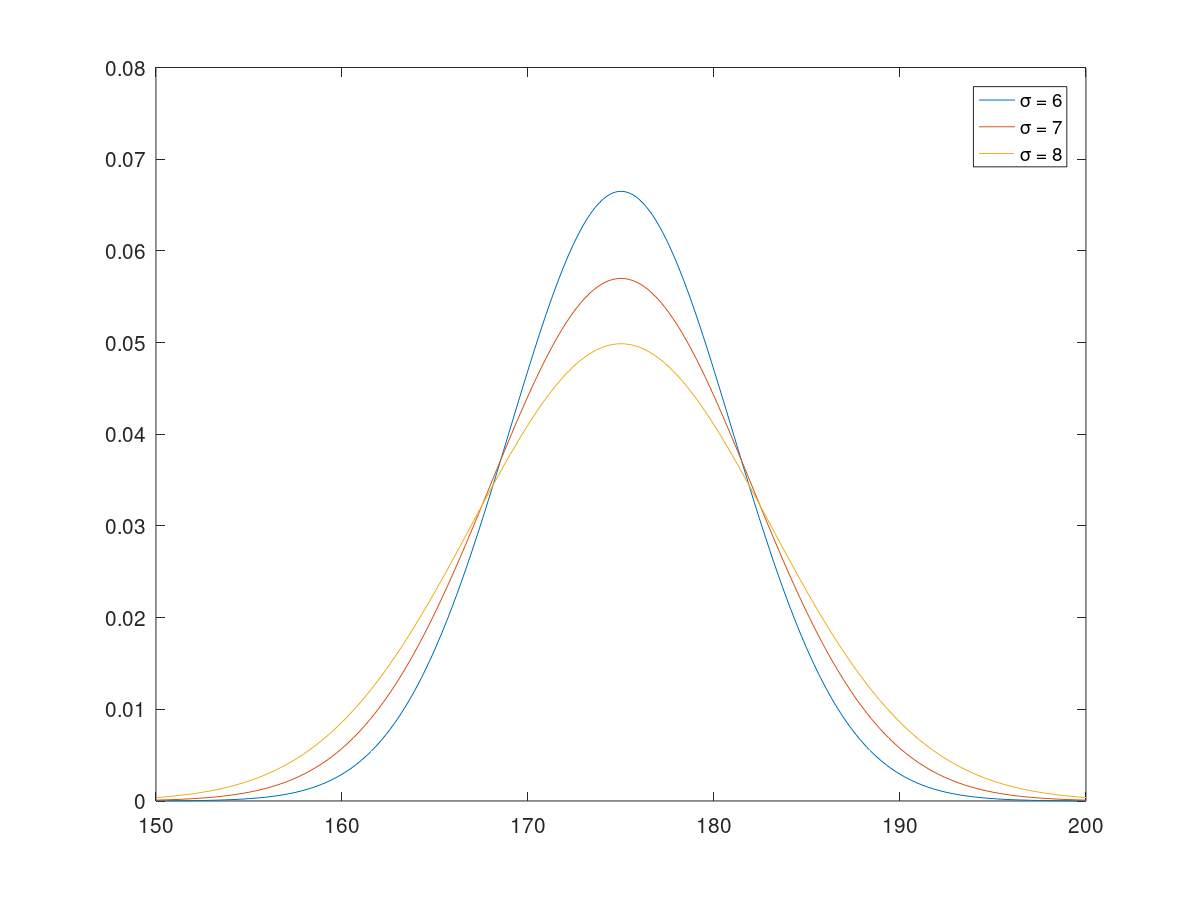
\includegraphics[width=\textwidth]{the2_plot.png}

The probability density functions all have the same mean of 175, while their
standard deviations are different. As the standard deviation increases, the
probabilites of values closer to the mean decreases and the probabilities of
values further from the mean increases.

\newpage

\subsection*{c)}

The probability of an adult having a height between 170 cm and 180 cm is
$0.5249$ as found in Answer 3. Therefore, among 150 randomly selected adults,
the probability that at least 45\%, 50\%, or 55\% of them having heights between
170 cm and 180 cm is binomially distributed, with parameters $n = 150$, and $p =
0.5249$. Normal approximation has parameters $\mu = 78.7424$, and $\sigma =
\sqrt{37.4066} = 6.1161$. For continuity correction, in the 50\% case, we are
going to use 75.5 instead.

\begin{align*}
  \boldP\{X > 150 \cdot 0.45\}
    &= \boldP\{X > 67.5\} \\
    &= \boldP \left\{ \frac{X - 78.74}{6.12}
                    > \frac{67.5 - 78.74}{6.12} \right\} \\
    &= \boldP \left\{ \frac{X - 78.74}{6.12}
                    > \frac{-11.24}{6.12} \right\} \\
    &= \boldP \left\{ \frac{X - 78.74}{6.12} > -1.84 \right\} \\
    &= 1 - \boldP \left\{ \frac{X - 78.74}{6.12} < -1.84 \right\} \\
    &= 1 - \Phi(-1.84) \\
    &= \Phi(1.84) \\
    &= 0.9670 \\
\\
  \boldP\{X > 150 \cdot 0.50\}
    &= \boldP\{X > 75\} \\
    &= \boldP\{X > 75.5\} \\
    &= \boldP \left\{ \frac{X - 78.74}{6.12}
                    > \frac{75.5 - 78.74}{6.12} \right\} \\
    &= \boldP \left\{ \frac{X - 78.74}{6.12}
                    > \frac{-3.24}{6.12} \right\} \\
    &= \boldP \left\{ \frac{X - 78.74}{6.12} > -0.53 \right\} \\
    &= 1 - \boldP \left\{ \frac{X - 78.74}{6.12} < -0.53 \right\} \\
    &= 1 - \Phi(-0.53) \\
    &= \Phi(0.53) \\
    &= 0.7020 \\
\\ \\ \\ \\
  \boldP\{X > 150 \cdot 0.55\}
    &= \boldP\{X > 82.5\} \\
    &= \boldP \left\{ \frac{X - 78.74}{6.12}
                    > \frac{82.5 - 78.74}{6.12} \right\} \\
    &= \boldP \left\{ \frac{X - 78.74}{6.12}
                    > \frac{3.76}{6.12} \right\} \\
    &= \boldP \left\{ \frac{X - 78.74}{6.12} > 0.61 \right\} \\
    &= 1 - \boldP \left\{ \frac{X - 78.74}{6.12} < 0.61 \right\} \\
    &= 1 - \Phi(0.61) \\
    &= \Phi(-0.61) \\
    &= 0.2695
\end{align*}

\noindent
This was the theoretical part. Now, we will conduct experiments and compare our
results with theoretical estimations. The Octave code is on the next page.

\newpage

\noindent
The Octave code is as follows,
\begin{lstlisting}[language=Octave]
  % Load statistics module for normal probability density function
  pkg load statistics;

  % Define constants
  N = 1000;
  mean = 175;
  std_dev = 7;

  % Generate heights as a column vector
  heights = randn(N, 1);
  heights *= std_dev;
  heights += mean;

  % Create and print the histogram of heights
  hist(heights, 10);
  print("the2_hist", "-dpng");

  % Create and print the normal PDF's with various standard deviations
  x = 150:0.1:200;
  hold off;
  plot(x, normpdf(x, mean, 6), ";\\sigma = 6;");
  hold on;
  plot(x, normpdf(x, mean, 7), ";\\sigma = 7;");
  plot(x, normpdf(x, mean, 8), ";\\sigma = 8;");
  print("the2_plot", "-dpng");

  % Generate heights as a 150x1000 matrix
  heights = randn(150, N);
  heights *= std_dev;
  heights += mean;

  % Filter heights and sum the successes
  heights = (heights > 170) & (heights < 180);
  heights = sum(heights);

  % Calculate probabilities
  p1 = sum(heights > 67.5)/N
  p2 = sum(heights > 75)/N
  p3 = sum(heights > 82.5)/N
\end{lstlisting}

\noindent
with a screenshot of some outputs,

\begin{center}
  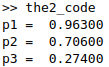
\includegraphics[scale = 1]{the2_outputs.png}
\end{center}

\noindent
The findings agree with our calculations. As the number of iterations increases,
the probabilities are expected to approach their theoretical values.

\end{document}